\section{Experimental Results}
\label{sec:moe_results}

We demonstrate the efficacy of the MoE controller in simulation
and real-world experiments.
%
In the first case study, we learn a gating network that switches between two
marginally stable closed-loop systems to result in a
piecewise-asymptotically-stable system.
%
Then, we find switching MoE controller to swing up the classical cartpole
mechanism enclosed with wall barriers.
%

\subsection{Switching Linear System}

We find the stable switching scheme through the MoE framework discussed in
Section~\ref{sec:motiviational_application}.
%
We aim to learn the parameters $\psi$ of the gating network $\mathbf{P}(x|
\psi)$ and the expert parameters $\theta_i$ such that the switching system
converges to the desired equilibrium $x^* = (0, 0)$.
%
The gating network is a fully-connected neural net with one hidden layer (2 input states 
$\rightarrow$ 6 hidden neurons $\rightarrow$ 4 outputs) and an \textsc{Elu} activation
function~\cite{clevert2015fast}.
%
We constrain the maximum number of state partitions to $N_F=4$.
%
Each state partition has a corresponding controller parameter $\theta_i \in
\mathbb{R}$. 
%

The response of the learned switching system is shown in
Figure~\ref{fig:final_switching}.
%
Figure~\ref{final_switching_control} shows the single best expert $F_a$
given by~\eqref{eq:best_expert_prediction} in each state partition, where purple
corresponds to $F_a=0$ or $\dot{x} = A_1x$ and yellow corresponds to $F_a=1$ or
$\dot{x} = A_2x$. The sample trajectory starts at $x_0=[-5, -5]$ and
successfully converges to the origin shown by the red star.
%
The state partition index of the single best expert is shown in
Figure~\ref{final_state_partition}, and it depicts that the training uses only 3
out of the 4 state partitions available.
%
The partitions in Figure~\ref{final_state_partition} matches the analytical
solution to the successful stable switching system given
by~\cite{liberzon2003switching}
\begin{equation*}
    \dot{x} = \begin{cases}
        A_1x, \; x_1x_2 \leq 0, \\
        A_2x, \; x_1x_2 > 0,
    \end{cases}
\end{equation*}
\noindent where $x=[x_1, x_2]$.
%
\begin{figure}[tb]
    \centering
    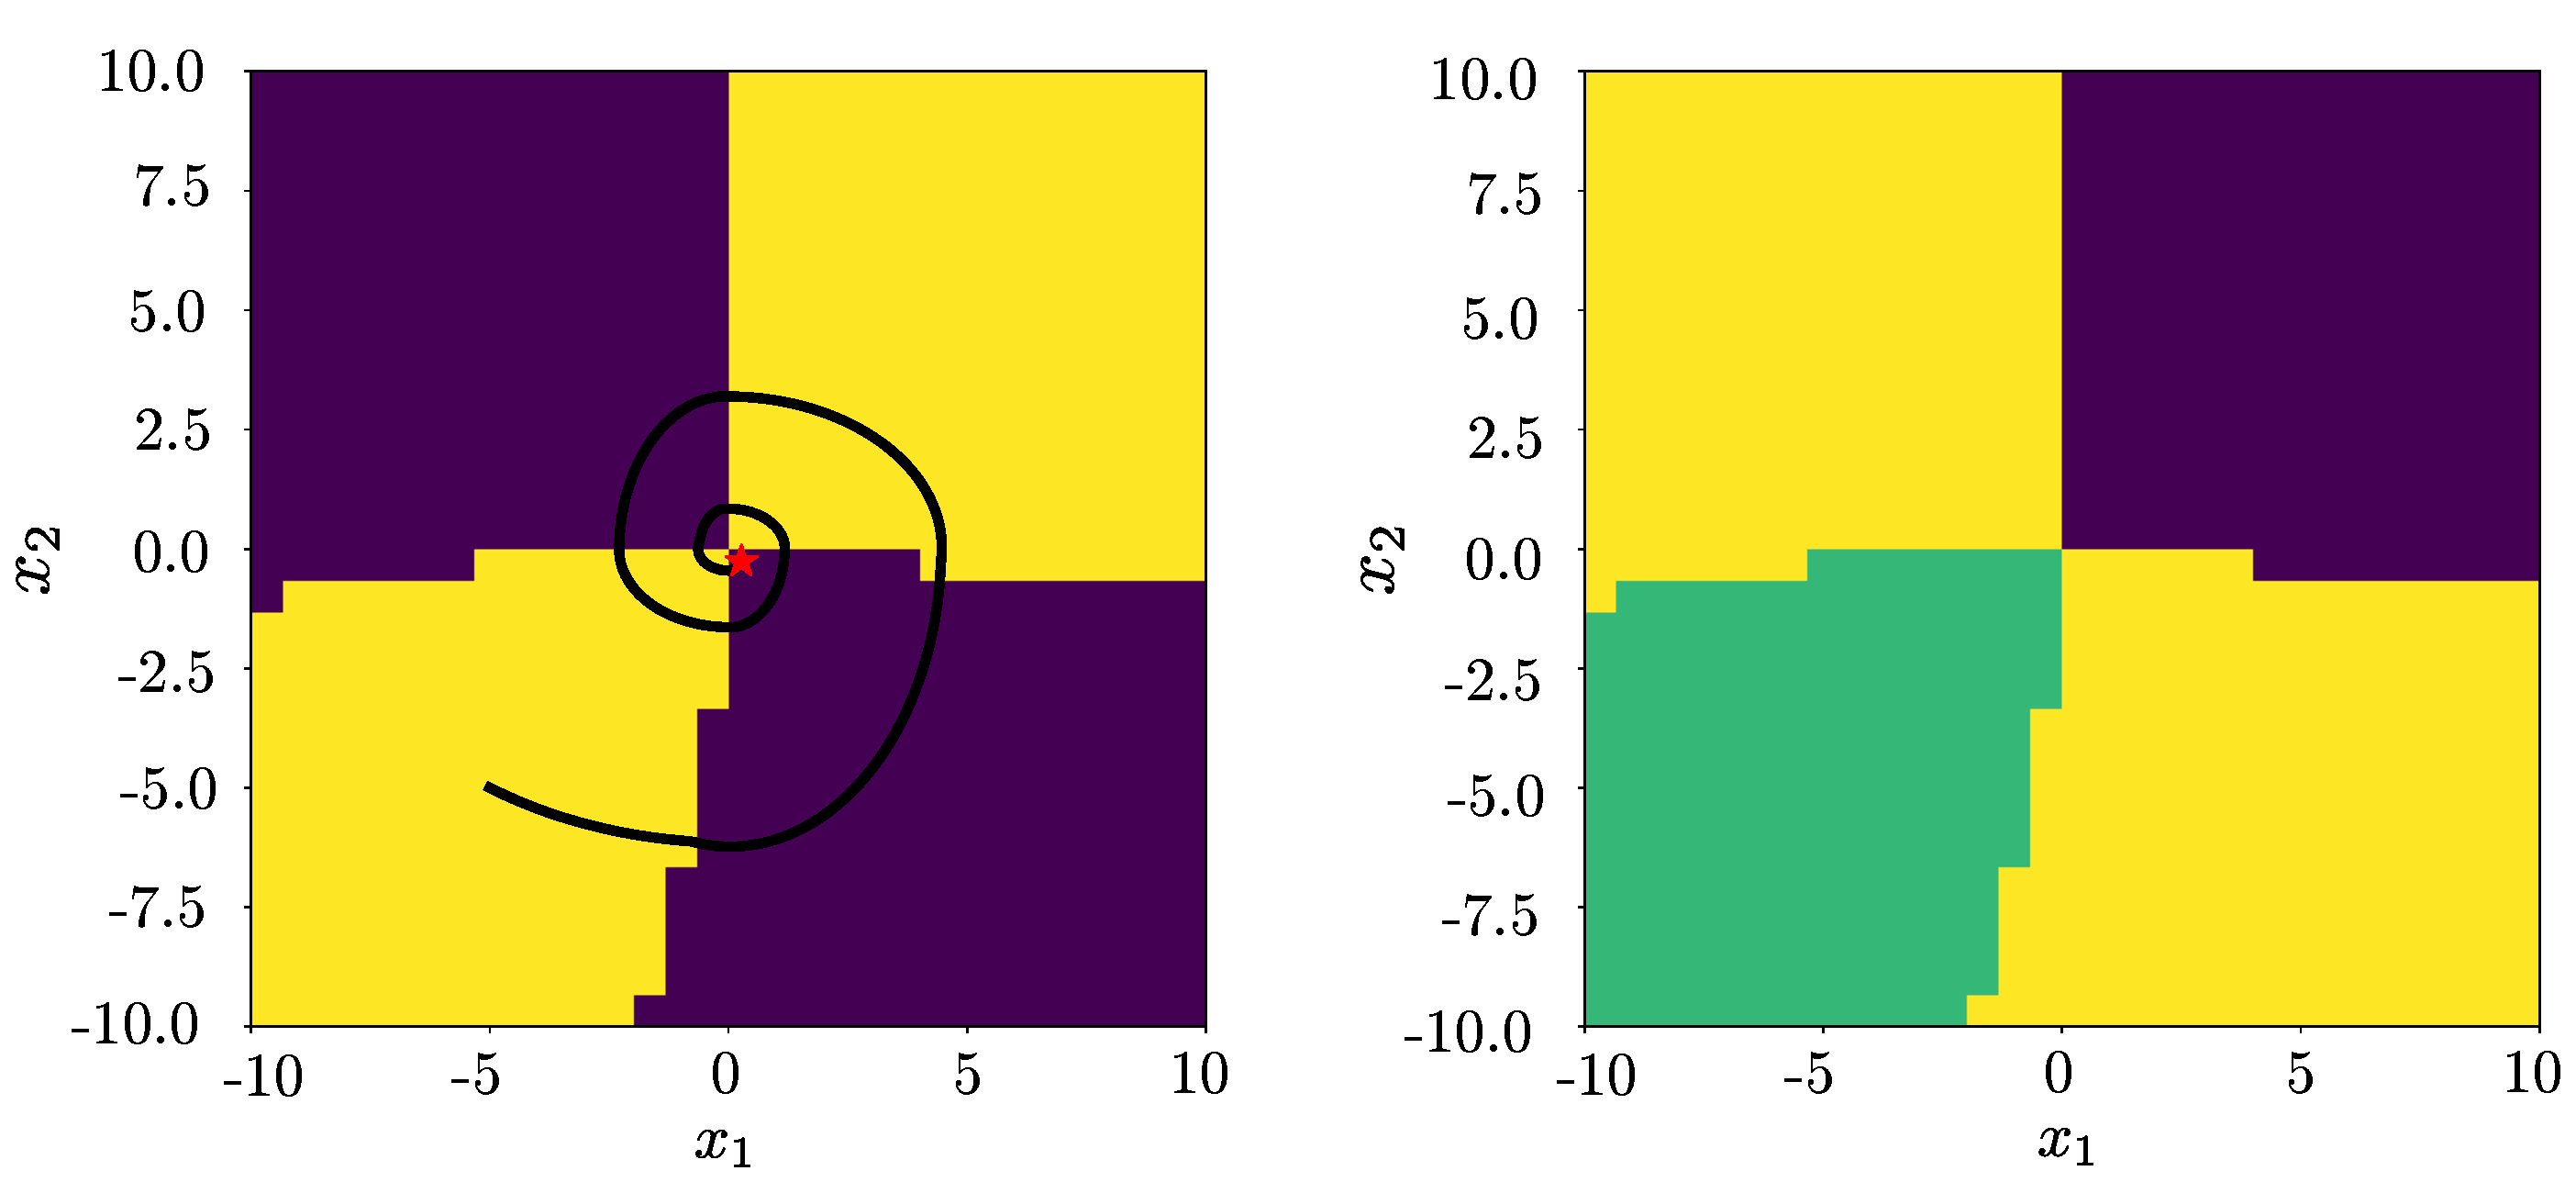
\includegraphics[width=0.9\linewidth]{switching_results.eps}
    \subfloat[\label{final_switching_control}]{\hspace{0.55\linewidth}} \subfloat[\label{final_state_partition}]{\hspace{0.4\linewidth}}
    \caption{Final stable switching system: (a) The single best expert $F_a$ in
    each state partition, where purple corresponds to $F_a=0$ or $\dot{x} =
    A_1x$ and yellow corresponds to $F_a=1$ or $\dot{x} = A_2x$, (b) State
    partition index of the single best expert}
    \label{fig:final_switching}
\end{figure}

%
\begin{figure}[tb]
    \centering
    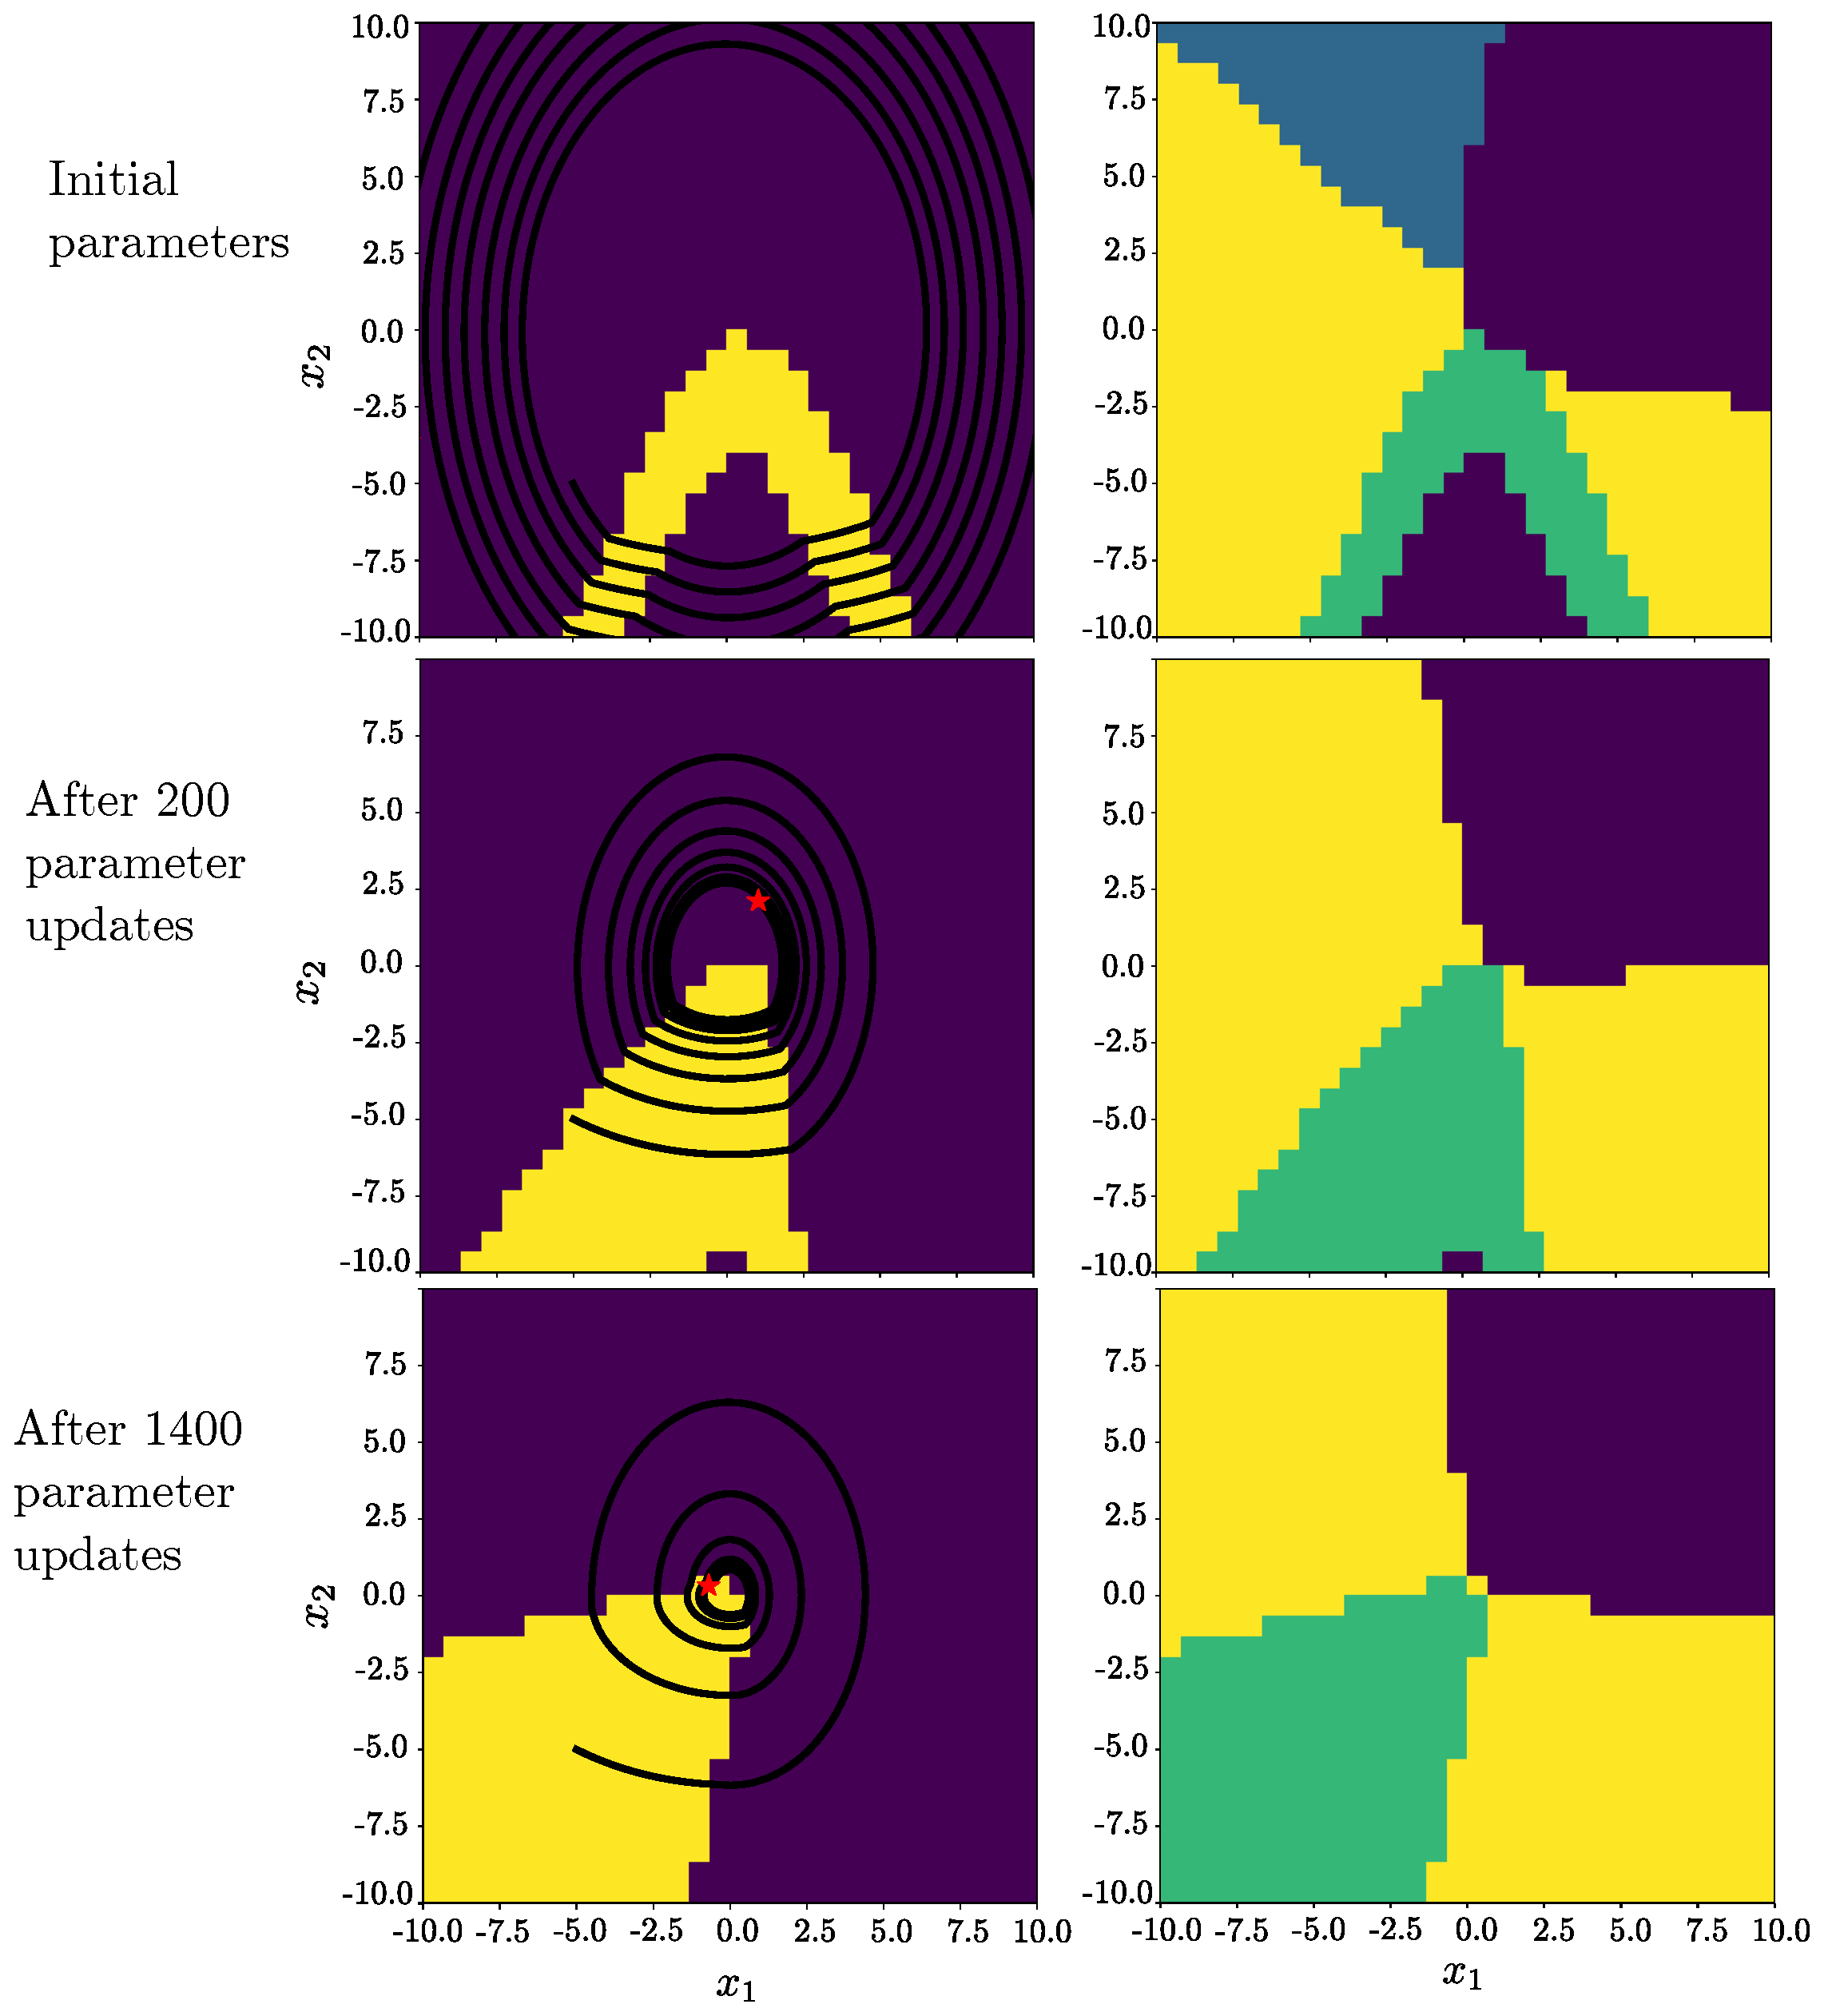
\includegraphics[width=0.65\linewidth]{switching_training.eps}
    \subfloat[\label{training_progress_control}Single best expert]{\hspace{0.4\linewidth}}
    \subfloat[\label{training_progress_partition}State partition index]{\hspace{0.3\linewidth}}
    \caption{Training progress. The final solution is shown in
    Figure~\ref{fig:final_switching}}
    \label{fig:switching_training}
\end{figure}
%
The training progress is shown in Figure~\ref{fig:switching_training}.
%
The three rows in the figure depict the performance of the training after 0, 200
and 1400 parameter updates, respectively.
%
The sample trajectory in Figure~\ref{training_progress_control} shows that the
initial parameters result in unstable switching between the two systems.
%
After only 200 parameter updates, the training finds a stable switching
mechanism, but it does not yet converge to the desired equilibrium $x^*$.
%
In order to create an asymptotically stable system, the corners of each state
partition must intersect at the origin, which the training finds successfully
after 2000 parameter updates (Figure~\ref{fig:final_switching}).
%
This is thanks to the explorative state sampling technique, which samples states
close to the desired equilibrium, assisting the training in finding the distinct
boundaries of each partition at the origin. 
%


%%%%%%%%%%%%%%%%%%%%%%%%%%%%%%%%%%%%%%%%%%%%%%%%%%%%%%%%%%%%%%%%%%%%%%%%%%%%%%%%%%%%%%%%
\subsection{Cartpole with Wall Contacts}
\label{ssec:cartpole_with_walls}

In this section, we take the classical cartpole swing-up problem and introduce
potential contacts from two barriers as shown Figure~\ref{fig:cartpole_contact}. 
%
The potential contacts serve as a way to convert the standard cartpole system
into a multi-modal dynamics.
%
The objective is to swing-up the pendulum on the cart in the presence of
contacts and impacts.
%
We apply the MoE framework to train switching expert controllers and a gating
network that governs the switching scheme.
%
We demonstrate the performance of the mixture of expert controller in
simulation and real-world experiments.
%
Lastly, we compare the performance of the MoE controller against
a single swing-up controller. 


\subsubsection{System Model}
\label{sssec:cartpole_model}

The cartpole system consists of a freely rotating pendulum link hinged on an
actuated cart.
%
The setup is enclosed by two rigid walls hanging $0.2$m from the bottom of the
cart.
%
The objective is to use the control authority on the cart in order to swing-up
the passive pendulum to the upright.
%
The pendulum spans length of $l=0.2$m and its mass $m_p = 0.75$kg is
concentrated at the distance $l_{cm}=\nicefrac{l}{2}$ from the hinge.
%
The cart alone has a mass of $m_c=0.165$ kg. The viscous friction in the cart
wheels is characterized by the coefficient $b=1.2$ \nicefrac{N $\cdot$ sec}{m}.
%
The dynamics of the system is given by~\eqref{eq:hybrid_dynamics} where 
%
\begin{align*}
    M(q) = \bmat{m_c + m_p & -m_p l_{cm} \cos(\theta_p) \\
    -m_pl_{cm}\cos(\theta_p) & m_p l_{cm}^2+I_p}, 
\end{align*}
\begin{equation}
    \begin{gathered}
    C(q, \dot{q}) = \bmat{b  & m_pl_{cm}\dot{\theta}_p\sin(\theta_p) \\
        0 & 0}, \\
    G(q) = \bmat{0 & -m_pg l_{cm} \sin(\theta_p)}^\top, \\
        B = [1 \; 0]^\top,
    \end{gathered}
\end{equation}
\noindent where $q = (x_c, \theta_p)$, $x_c$ is the location of the cart,
$\theta_p$ is the angle of the pendulum from the vertical. The moment of inertia
of the pendulum is given by $I_p$ and $g$ is the acceleration due to gravity. 
%
There are a total of $k=10$ potential contacts between the pendulum and the sides of
the walls.
%
We integrate closed-loop trajectories with Moreau time stepping algorithm
outlined in Algorithm~\eqref{algo:moreau} with an integration time step $\Delta
t=0.001$.
%
% \begin{figure}[tb]
%     \centering
%     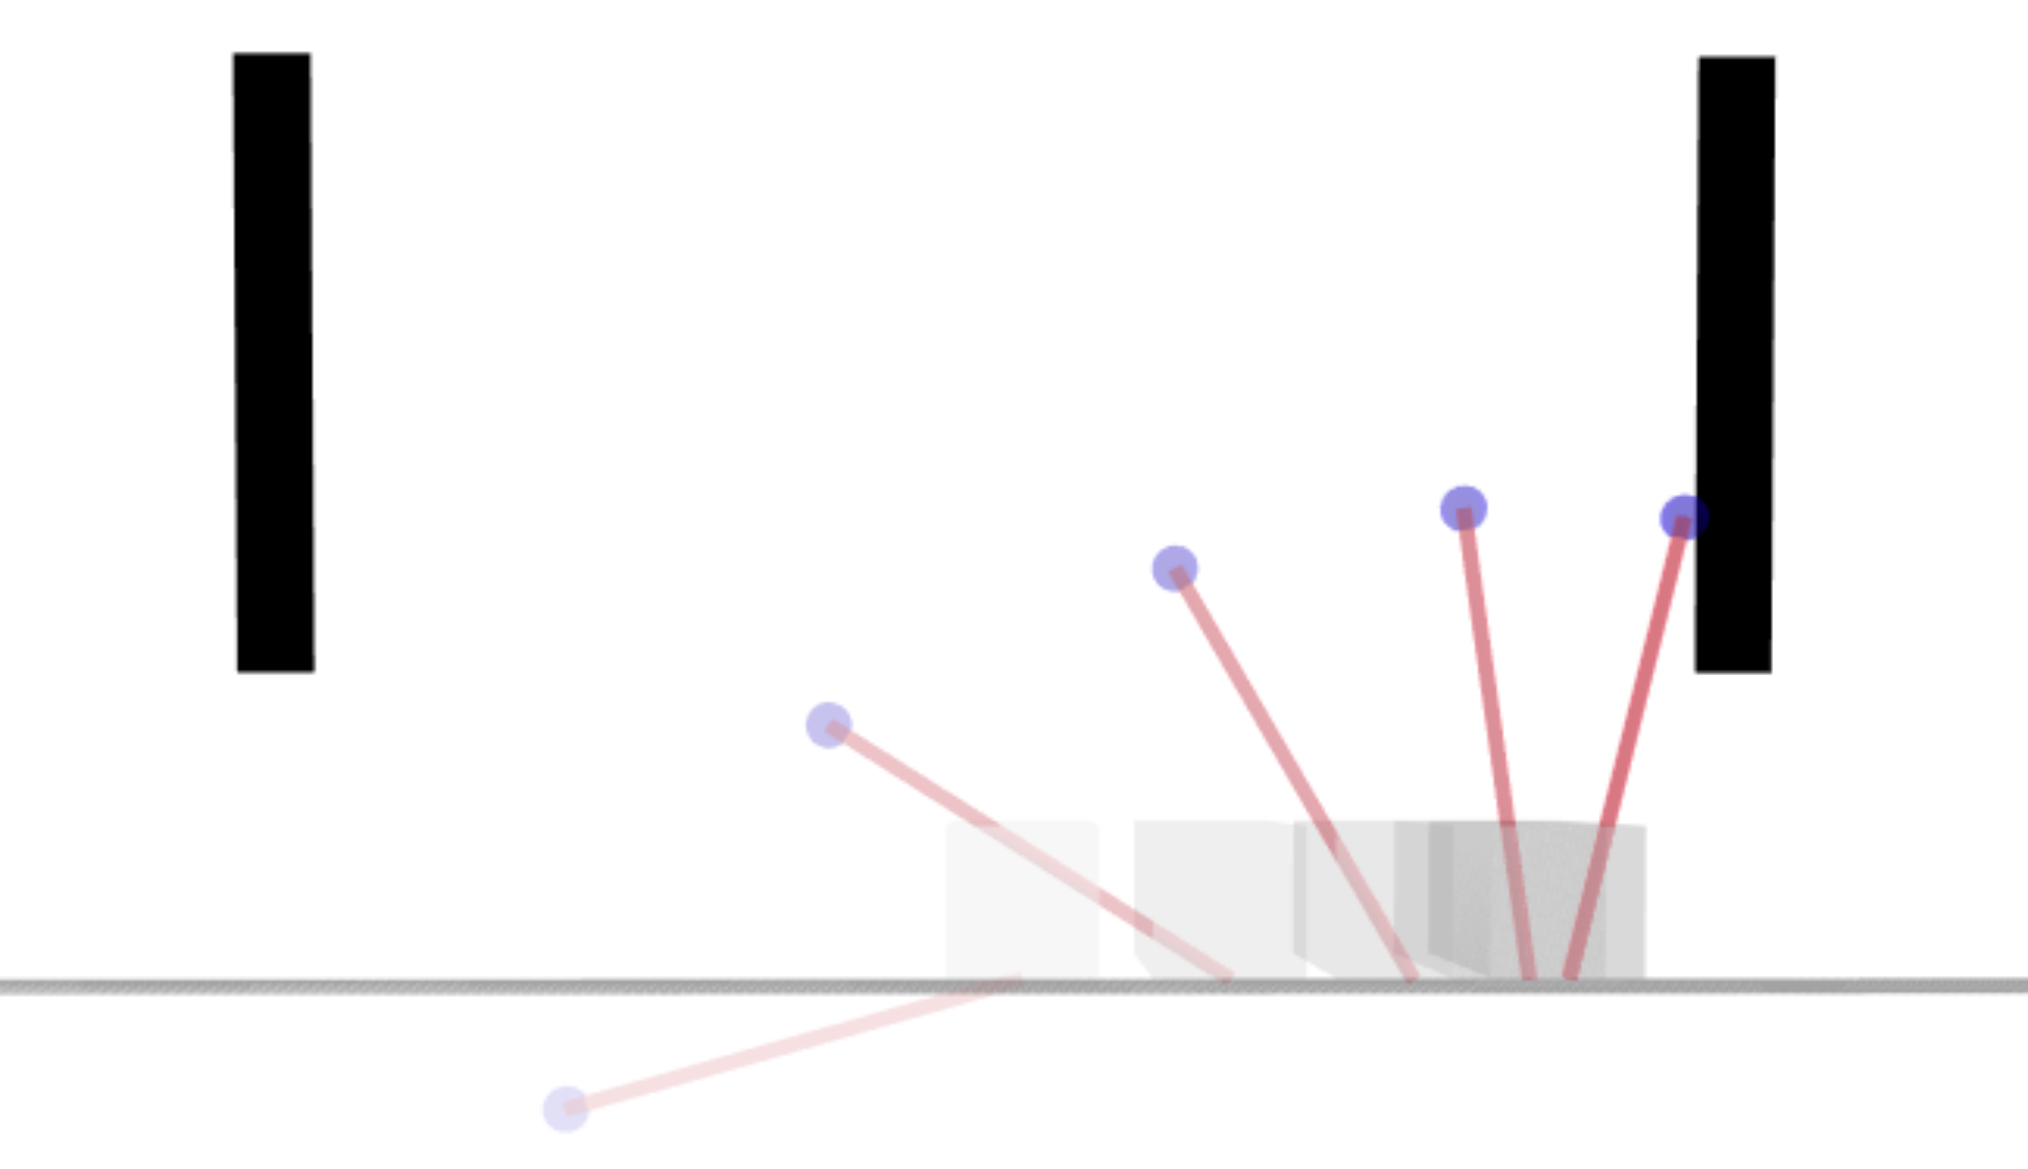
\includegraphics[width=0.6\linewidth]{MOEfirstImpact.png}
%     \caption{Cartpole with wall contacts}
%     \label{fig:cartpole_contact}
% \end{figure}
\begin{figure}[tb]
    \centering
    \begin{tikzpicture}
    
        \node [](image) at (0,0) {
            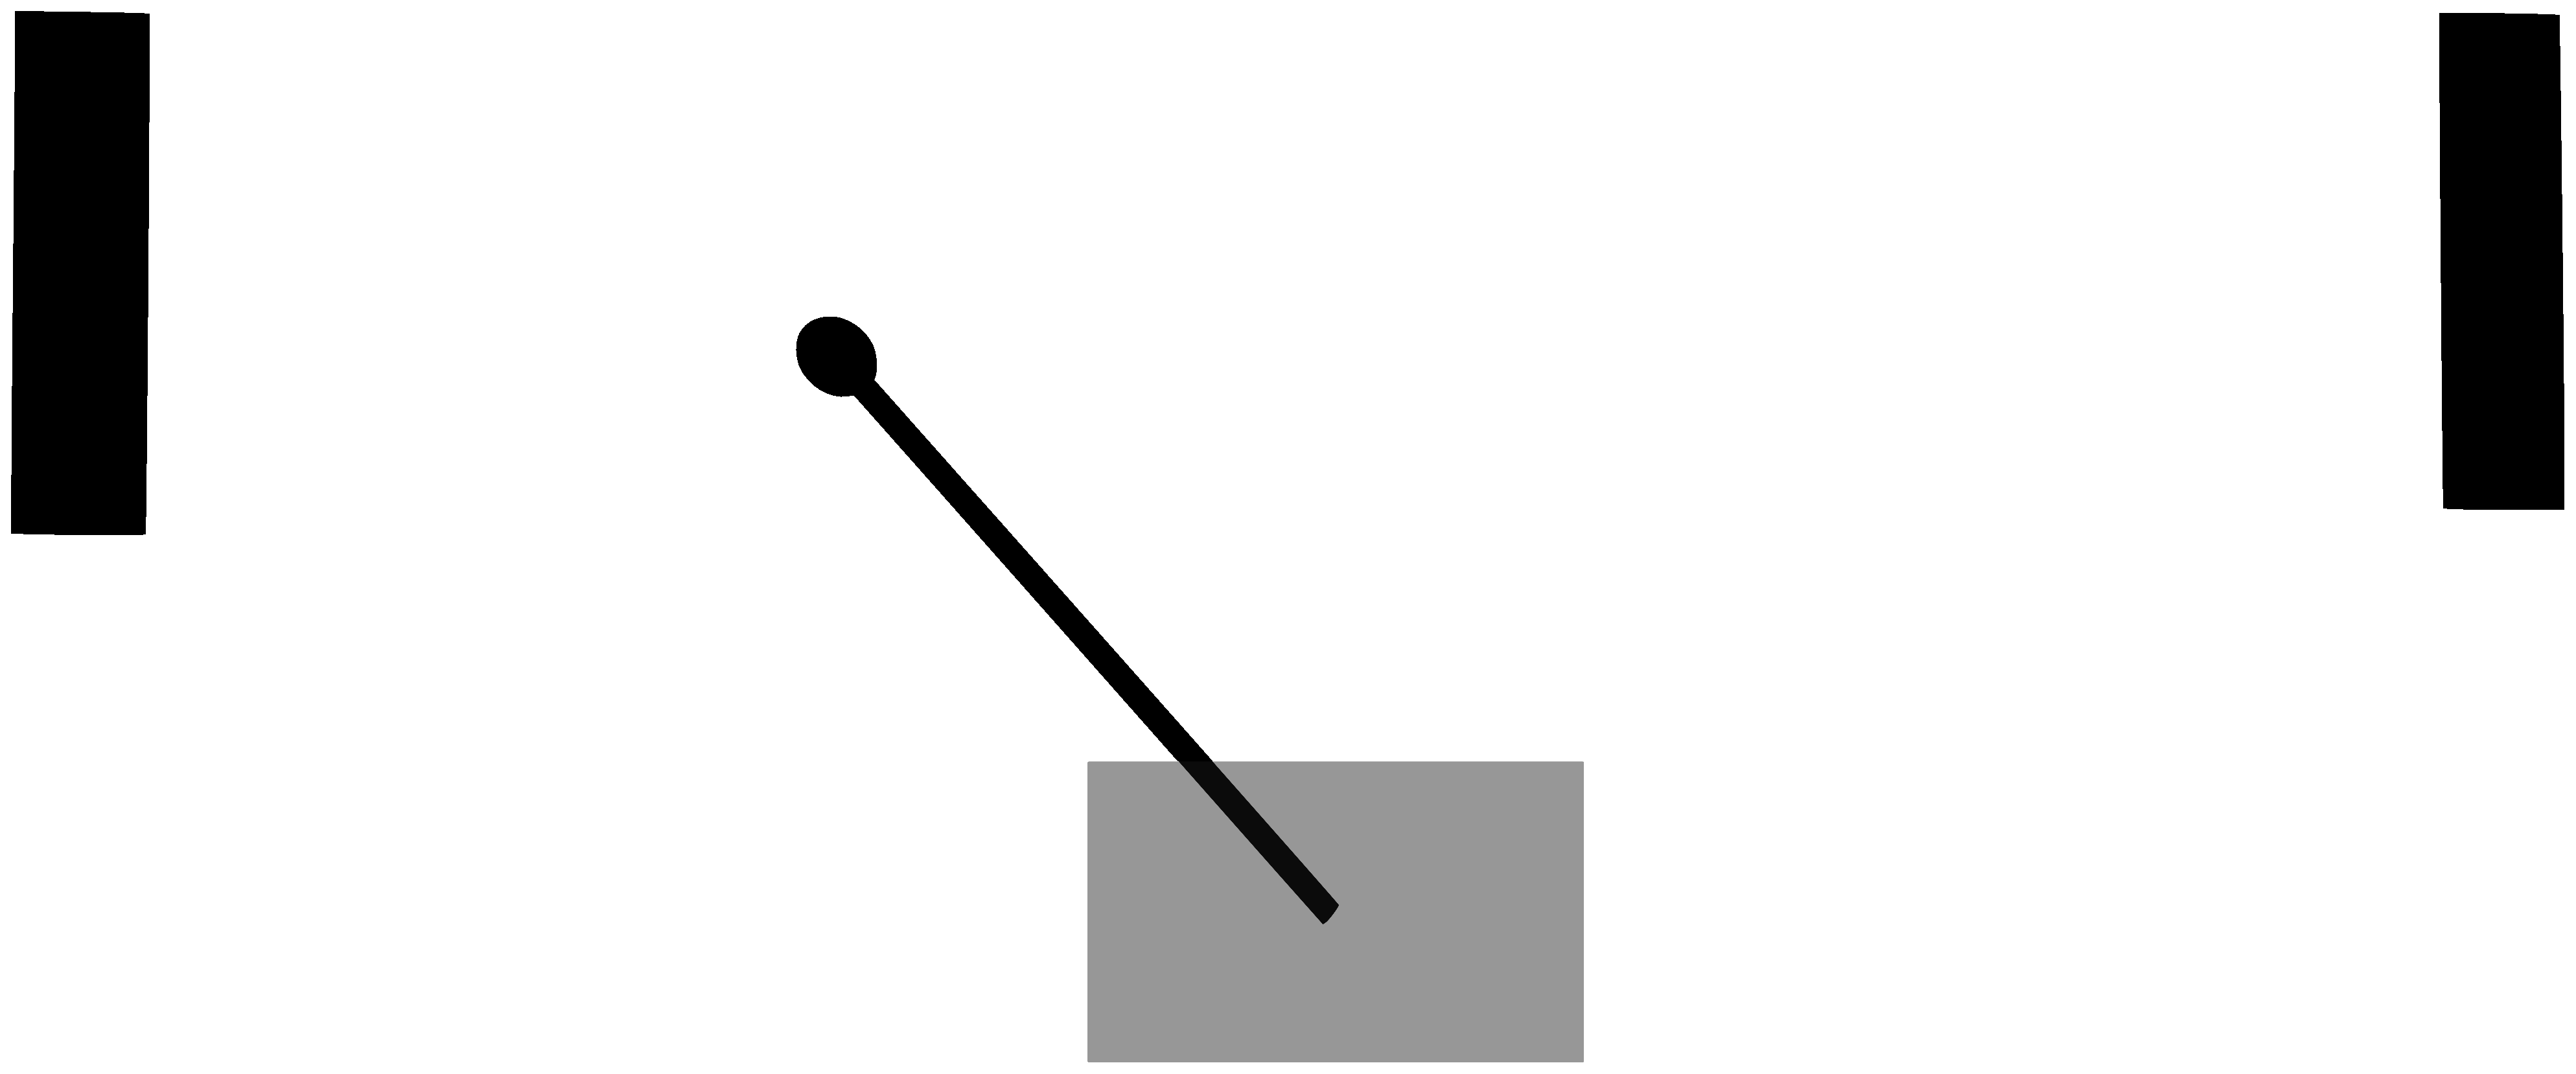
\includegraphics[width=0.5\textwidth]{cartpole_sketch2.eps}
        };
        \draw[dotted, very thick,black] (0.1,-1.8) -- ++(0.0,4.0);
        \draw[-stealth, very thick,black]  (0.1,0.0) arc (90:135:1); 
        \node[] at (-0.3,0.3) {\small $\theta_p$};
        \draw[-stealth, very thick,black] (0.1,1.1) -- ++(-3.5, 0.0) node[above right,black]{\small $\abs{d}=0.45$m};
        \draw[-stealth, very thick,black] (0.1,-1.1) -- ++(1.7, 0.0) node[above,black]{\small $x_c$};
    \end{tikzpicture}
    \caption{Cartpole with wall contacts}
    \label{fig:cartpole_contact}
\end{figure}

\subsubsection{Training}
\label{sssec:cartpole_training}

\begin{table}[b]
    \centering
    \small
    \caption{Structure of the deep-net experts and the gating network.\label{tab:neural-net-structure}}
    \begin{tabular}{|c|c|c|c|}
    \hline
    Neural Network & Inputs &  \begin{tabular}{@{}c@{}}Number of neurons \\ in hidden layers\end{tabular} & Outputs\\
    \hline
    Expert $F_i(x;\theta_i)$ & $[x_c, \cos(\theta_p), \sin(\theta_p), \dot{x}_c, \dot{\theta}_p]$ & (10, 4) & $u \in \mathbb{R}$\\
    Gating network $\mathbf{P}(x |\psi)$ & $[x_c, \cos(\theta_p), \sin(\theta_p), \dot{x}_c, \dot{\theta}_p]$ & (4, 3) & [$P_1, P_2, P_3$]\\ 
    \hline
  \end{tabular}
\end{table}
We aim to learn the parameters $(\psi, \theta)$ of the MoE controller in order to stabilize the 
cartpole system to the desired state $x^* = (q^*, \dot{q})^* =
((0, 0), (0, 0))$ under contacts, impacts and Coulomb friction.
%
Once the system reaches within a small neighborhood of $x^*$, we employ Linear
Quadratic Regulator (LQR) to maintain the system at the desired equilibrium.
%
The structures of the deep-net experts and gating network are provided in
Table~\ref{tab:neural-net-structure}.
%
% The gating network is a fully-connected
% neural net with two hidden layers (state input $\rightarrow$ 4 neurons
% $\rightarrow$ 3 neurons $\rightarrow$  3 output).
% 
We constrain the maximum number of state partitions to 3, where each partition
has a local expert $F_i$.
%
%
% The experts are fully-connected neural nets with two hidden layers (state input
% $\rightarrow$ 10 neurons $\rightarrow$ 4 neurons $\rightarrow$  1 output).
%
The output of the experts correspond to the force applied on the cart.
%
We use minimum trajectory loss (MTL) discussed in
Section~\ref{ssec:performance_objective} with time horizon $T=1.5$s, where the
performance metric $\ell$ is given by~\eqref{eq:accumulatedLoss}.
%
In each parameter update, we sample $N_{\mathcal{D}}=4$ initial states through
greedy and explorative techniques.
%


\subsubsection{Hardware}

%
We demonstrate the performance of the MoE controller in simulation and hardware. 
%
The hardware (Figure~\ref{fig:cartpole_hardware}), designed and built by
\textsc{Quanser}~\cite{Quanser_2021}, uses a DC-motor to translate the cart on a
track.
% 
The cart uses a rack-and-pinion mechanism to translate on the track with
zero-slip.
%
\begin{figure}[tb]
    \centering
    \begin{tikzpicture}
        \node [](image) at (0,0) {
            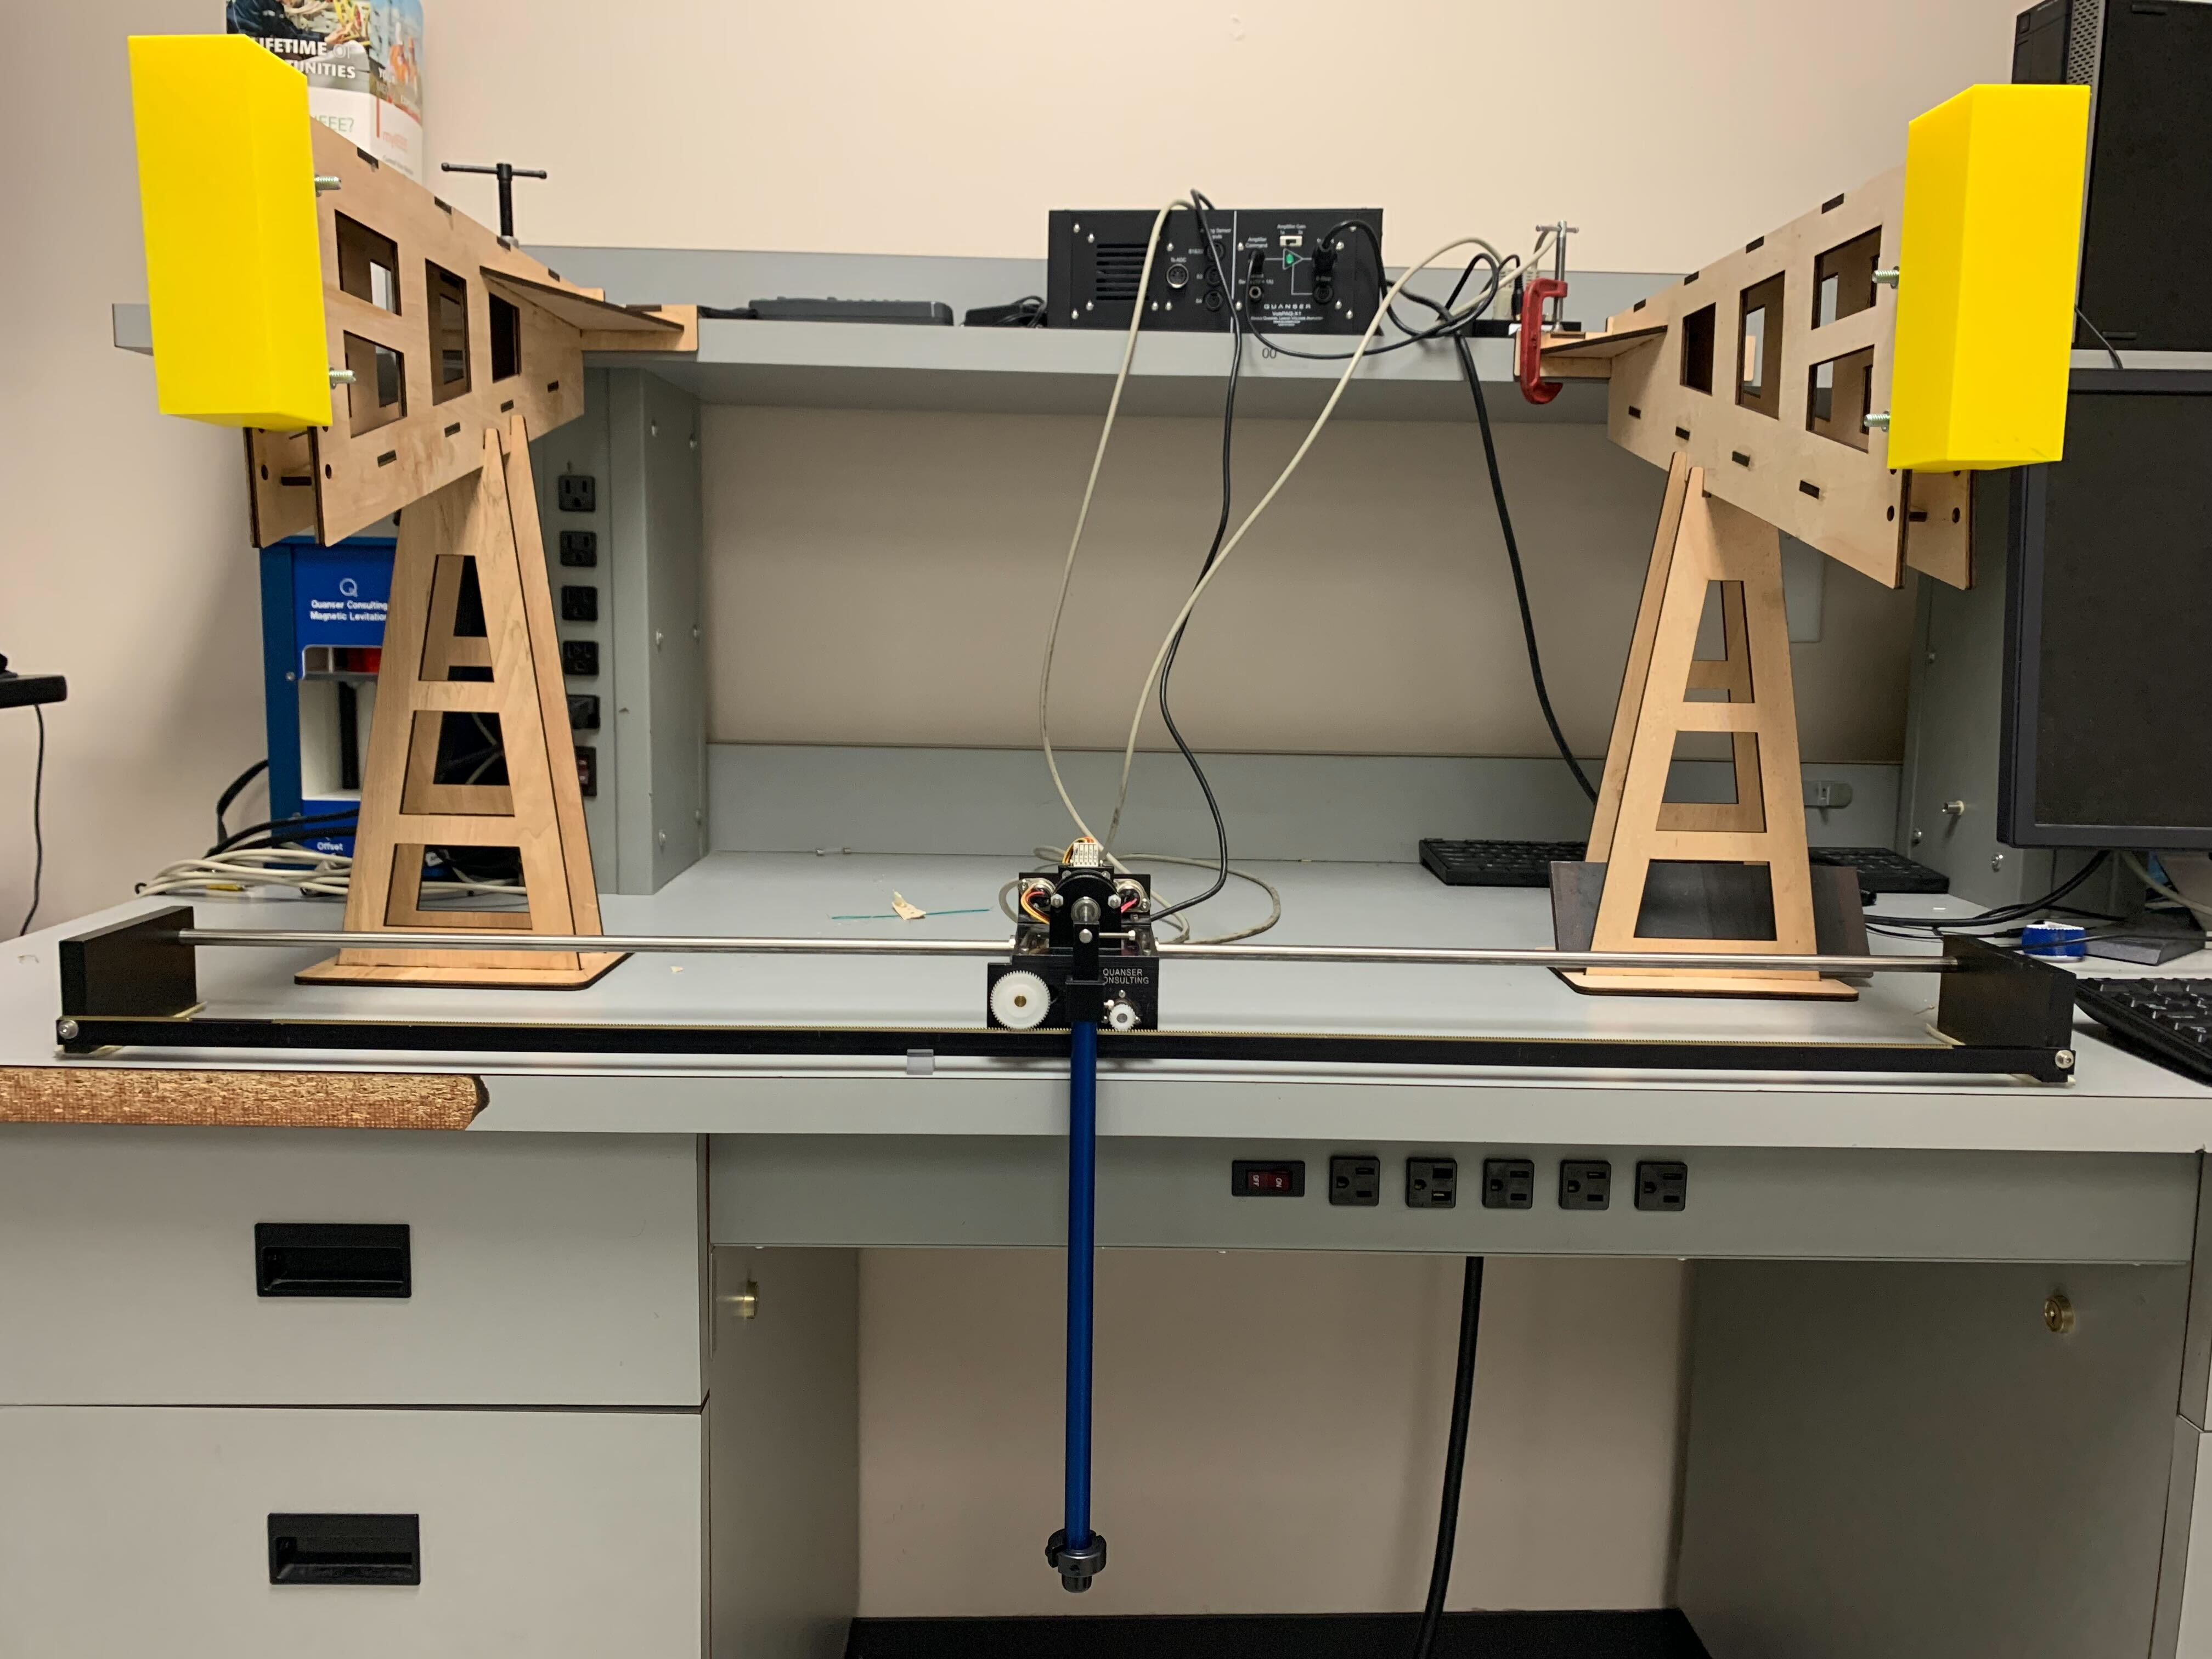
\includegraphics[width=0.65\textwidth]{cartpole_hardware_2.jpg}
        };
        \draw[stealth-, ultra thick,red] (-4.0,2.2) -- ++(-2.0, 0.0) node[left,black]{\small Left wall};
        \draw[stealth-, ultra thick,red] (4.0,2.0) -- ++(1.3, 0.0) node[right,black]{\small Right wall};
        \draw[stealth-, ultra thick,red] (-0.1,-2.0) -- ++(-5.8, 0.0) node[left,black]{\small Pendulum};
        \draw[stealth-, ultra thick,red] (2.0,-1.0) -- ++(4.0, 0.0) node[right,black]{\small Track}; 
        \draw[stealth-, ultra thick,red] (-0.1,-0.3) -- ++(-6.0, 0.0) node[left,black]{\small Cart};
    \end{tikzpicture}
    \caption{Experimental setup of cartpole with wall contacts}
    \label{fig:cartpole_hardware}
\end{figure}
%
One of the wheels of the cart is attached to an optical encoder, from which we
estimate the position and velocity of the cart.
%
There is also an optical encoder rigidly attached to the pendulum link,
reporting its orientation. 
%
We evaluate the experts and the gating network in MATLAB/Simulink and pass the
corresponding voltage commands to the DC-motor via \textsc{Quarc},
\textsc{Quanser's} real-time control software.
%
The force commands output by the MoE controller are converted into voltage
commands $V(t)$ as follows.
%
\begin{align*}
    V(t) = \frac{u(x(t)) + A_m \dot{x}_c(t)}{B_m},
\end{align*} 
\noindent where $A_m$ and $B_m$ consist of system parameters of the motor.
%


\subsubsection{Results}

Figure~\ref{fig:cartpole_trajectory} shows a successful swing-up trajectory
generated by the MoE controller in simulation and hardware.
%
The blue contours correspond to the level sets of the control input $u$ during
impact ($x_c=0.36m, \dot{x}_c = 0\nicefrac{m}{s}$), and the solid red lines
depict the boundaries of the state partitions.
%
Although the gating network can provide up to three state partitions,
the training converges to utilizing only two.
%
Figure~\ref{fig:cartpole_trajectory} shows that the system successfully avoids
contacts during the swing-up phase, which otherwise would have prevented the
pendulum from pumping energy from the downward equilibrium.
%
By the time the pendulum approaches the upright equilibrium, it is moving at
such high speed ($\sim$-6\nicefrac{rad}{s}) that LQR cannot stabilize the
pendulum to the upright.
%
However, we have observed from several trajectories that the system leverages
the impact from the wall to lower the speed of the pendulum.
%
During impact, the control law switches experts, where the new expert applies
rapid braking allowing the LQR to catch the pendulum post-impact.
%
The MoE controller achieves successful swing-up in simulation and real-world,
proving the accuracy in the contact model and the robustness of the
controllers.
\begin{figure}[tb]
    \centering
    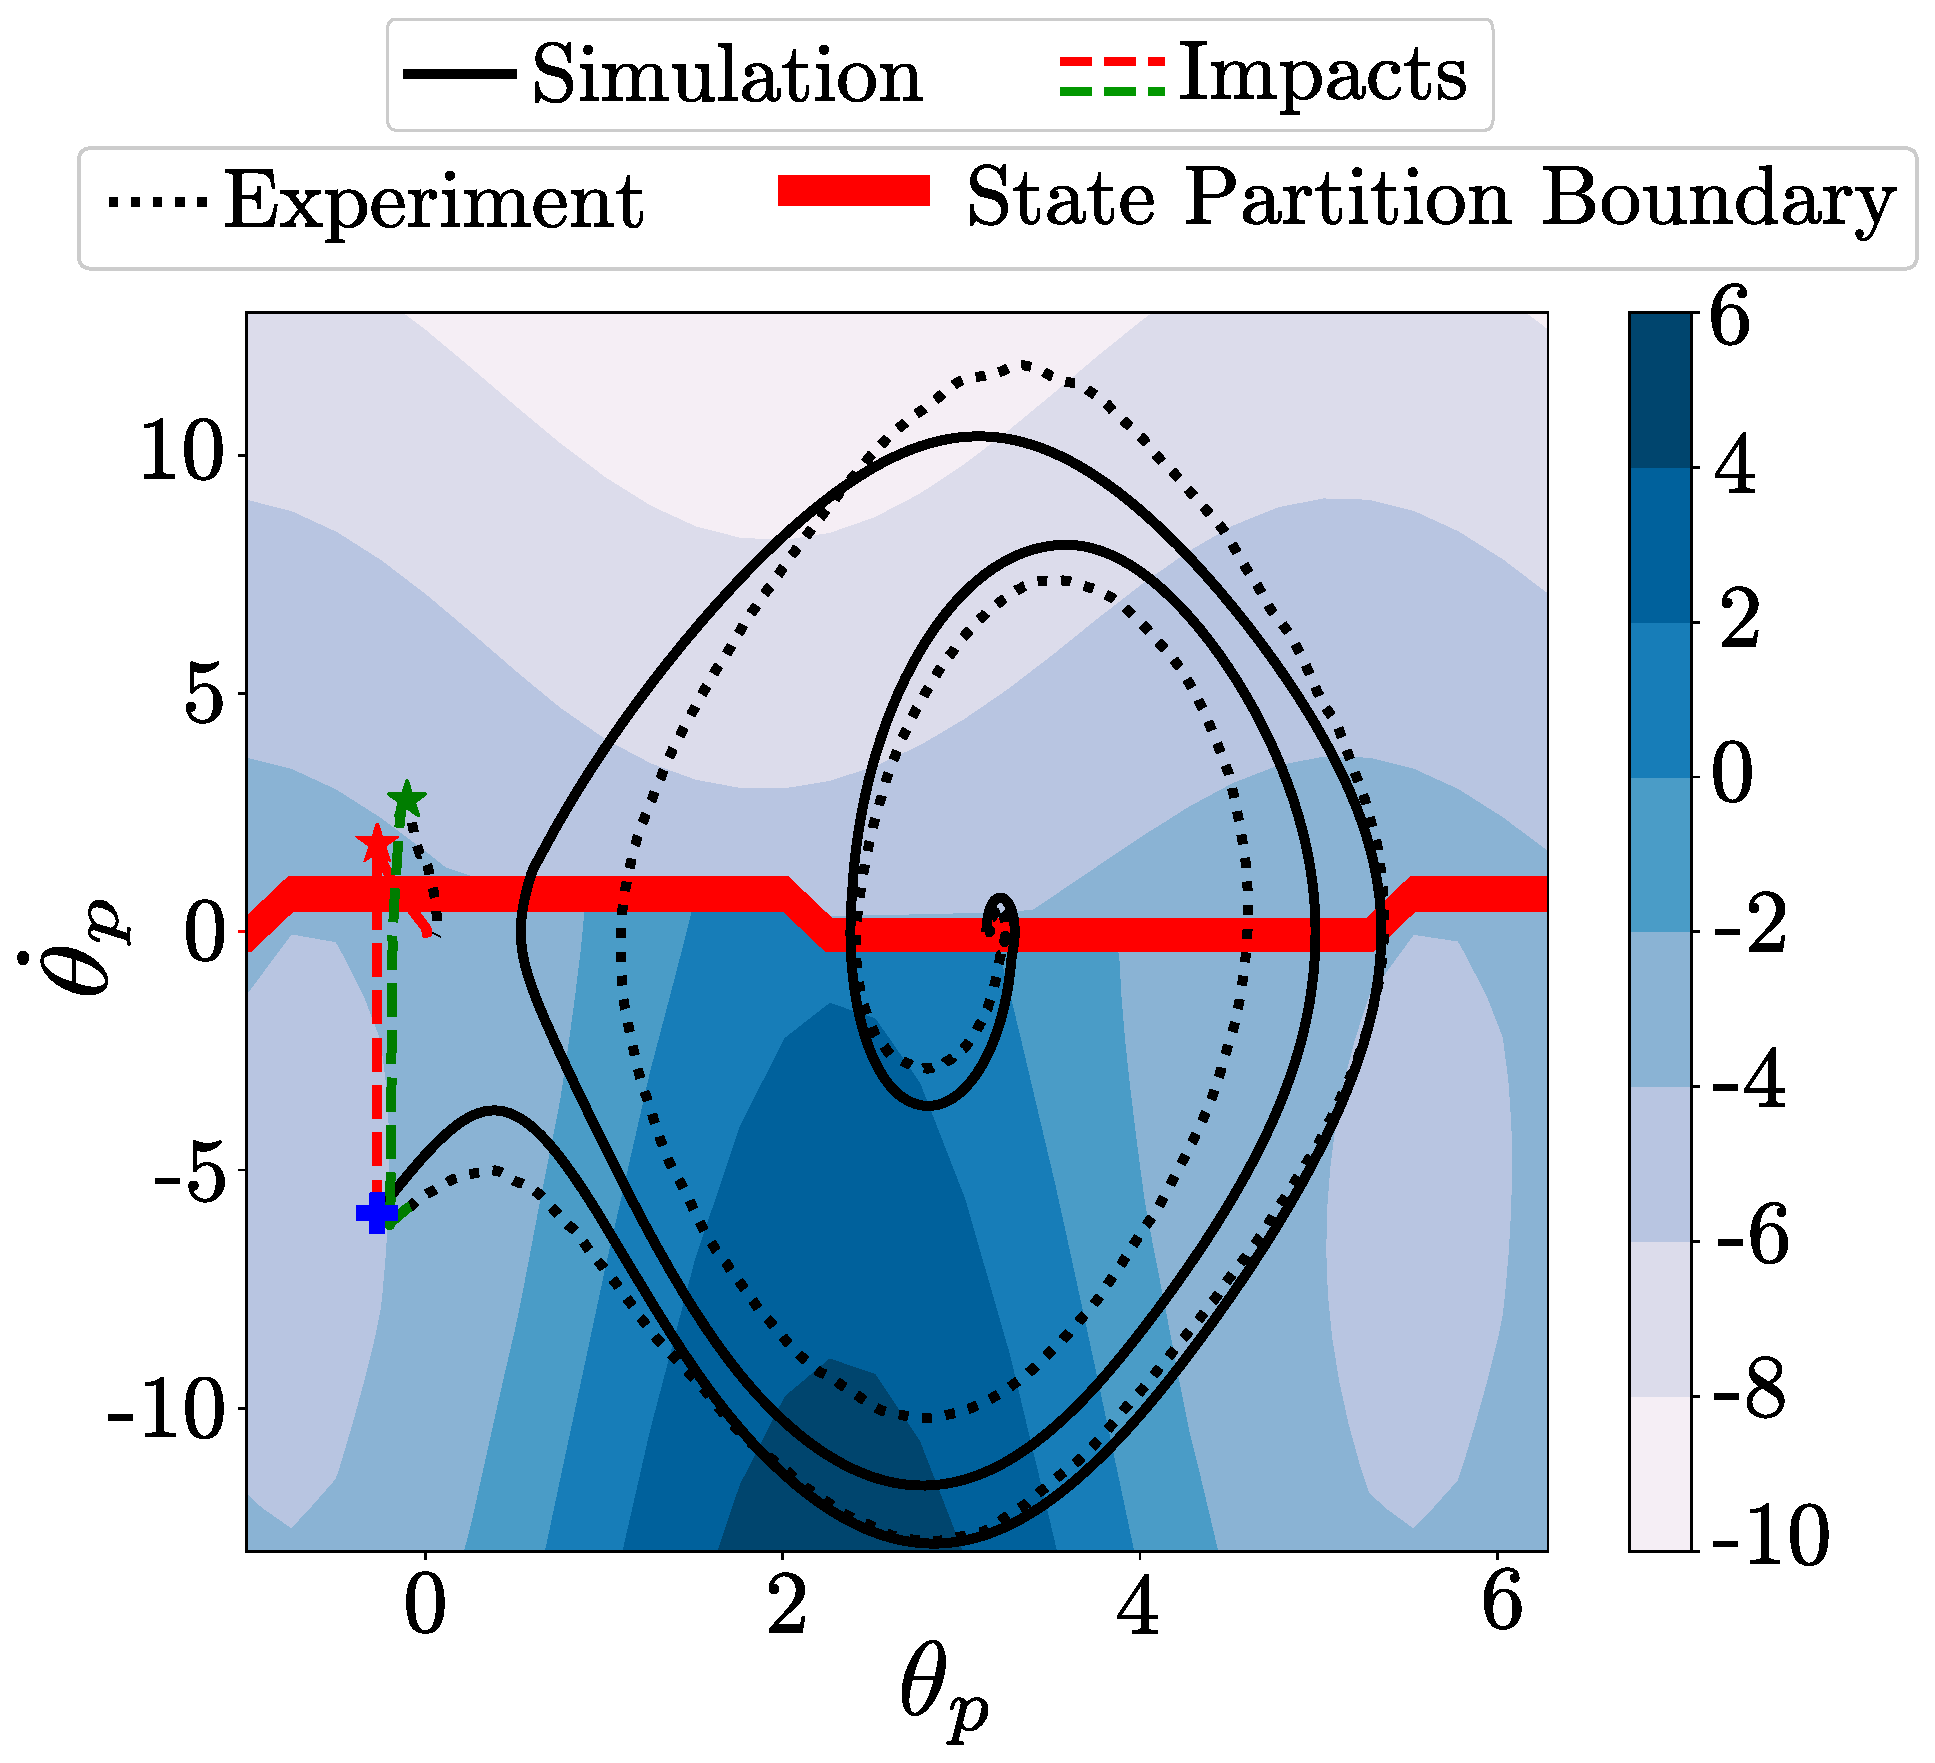
\includegraphics[width=0.5\linewidth]{moe_traj_red_boundaries.eps}
    \caption{A sample trajectory starting from
    downward equilibrium at rest. The blue contours represent the level sets of
    the control input at the pre-impact and post-impact states}
    \label{fig:cartpole_trajectory}
\end{figure}
% \begin{figure}[tb]
%     \centering
%     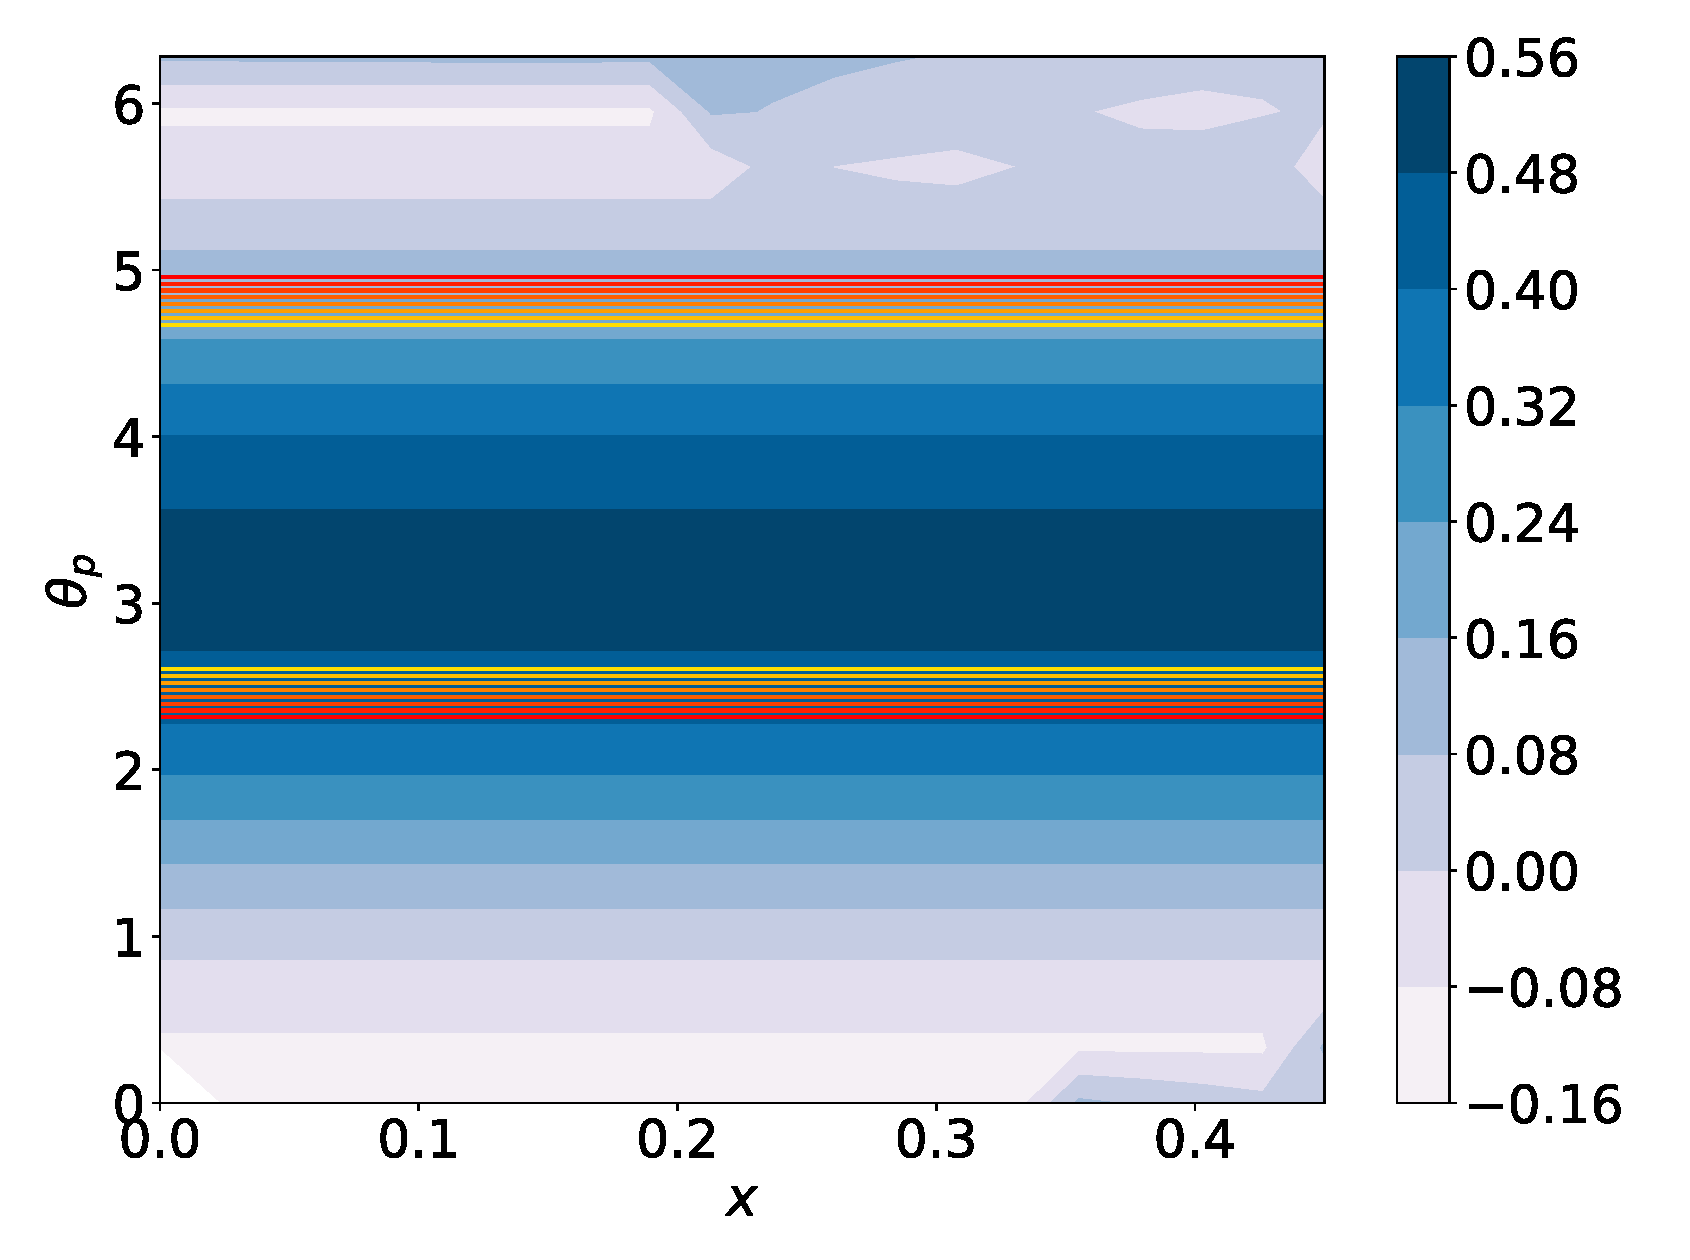
\includegraphics[width=0.7\linewidth]{gapContourAndBins.eps}
%     \caption{The blue contours represent the level sets of the gap function. The red lines show the boundaries of the state partition. There are a total of two experts, one is active between the red boundaries and the other is responsible for regions outside the red lines.}
%     \label{fig:gapContour}
% \end{figure}
% Figure~\ref{gap} shows the relationship between the selected expert and the
% occurrence of potential contacts.
% %
% The blue contours depict the level sets of the shortest gap between the pendulum and
% the walls.
% %
% The region enclosed by the red boundaries corresponds to the state partition $i=1$
% where local expert $F_1(x;\theta_1)$ is executed.
% %
% Conversely, expert $F_2(x;\theta_2)$ is responsible for regions outside the red
% boundaries.
% %
% Notice that the states in partition $i=1$ have large gap values, hence there are
% no potential contacts in this region.
% %
% This shows that the gating network has dedicated one expert for states with low
% risk of contact.
% %
% Expert $F_2(x;\theta_2)$ is responsible for states with high risk of contact and
% from the trajectory in Figure~\ref{control}, this expert prevents contact during the
% swing-up phase and catches the pendulum just after impact.
% %
% This demonstrates that the state partition depends on the occurrence of
% potential contacts, proving that the MoE controller provides the desirable
% characteristics of assigning specialized controllers to different modes of a
% hybrid system.
%

%
\textbf{Comparison between MoE and single controller}: We compare the
performance of the MoE controller against a single controller, which can be
thought of as the MoE controller with $N_F=1$.
%
This controller is parameterized by a neural net, with a similar structure to
the experts provided in Table~\ref{tab:neural-net-structure}.
%
We train the controller with the same minimum trajectory loss (MTL) and training
parameters as the MoE.
%
Once the controller swings the pendulum to the neighborhood of $x^*$, we use LQR
to stabilize it to the upright.

\begin{figure}[tb]
    \centering
    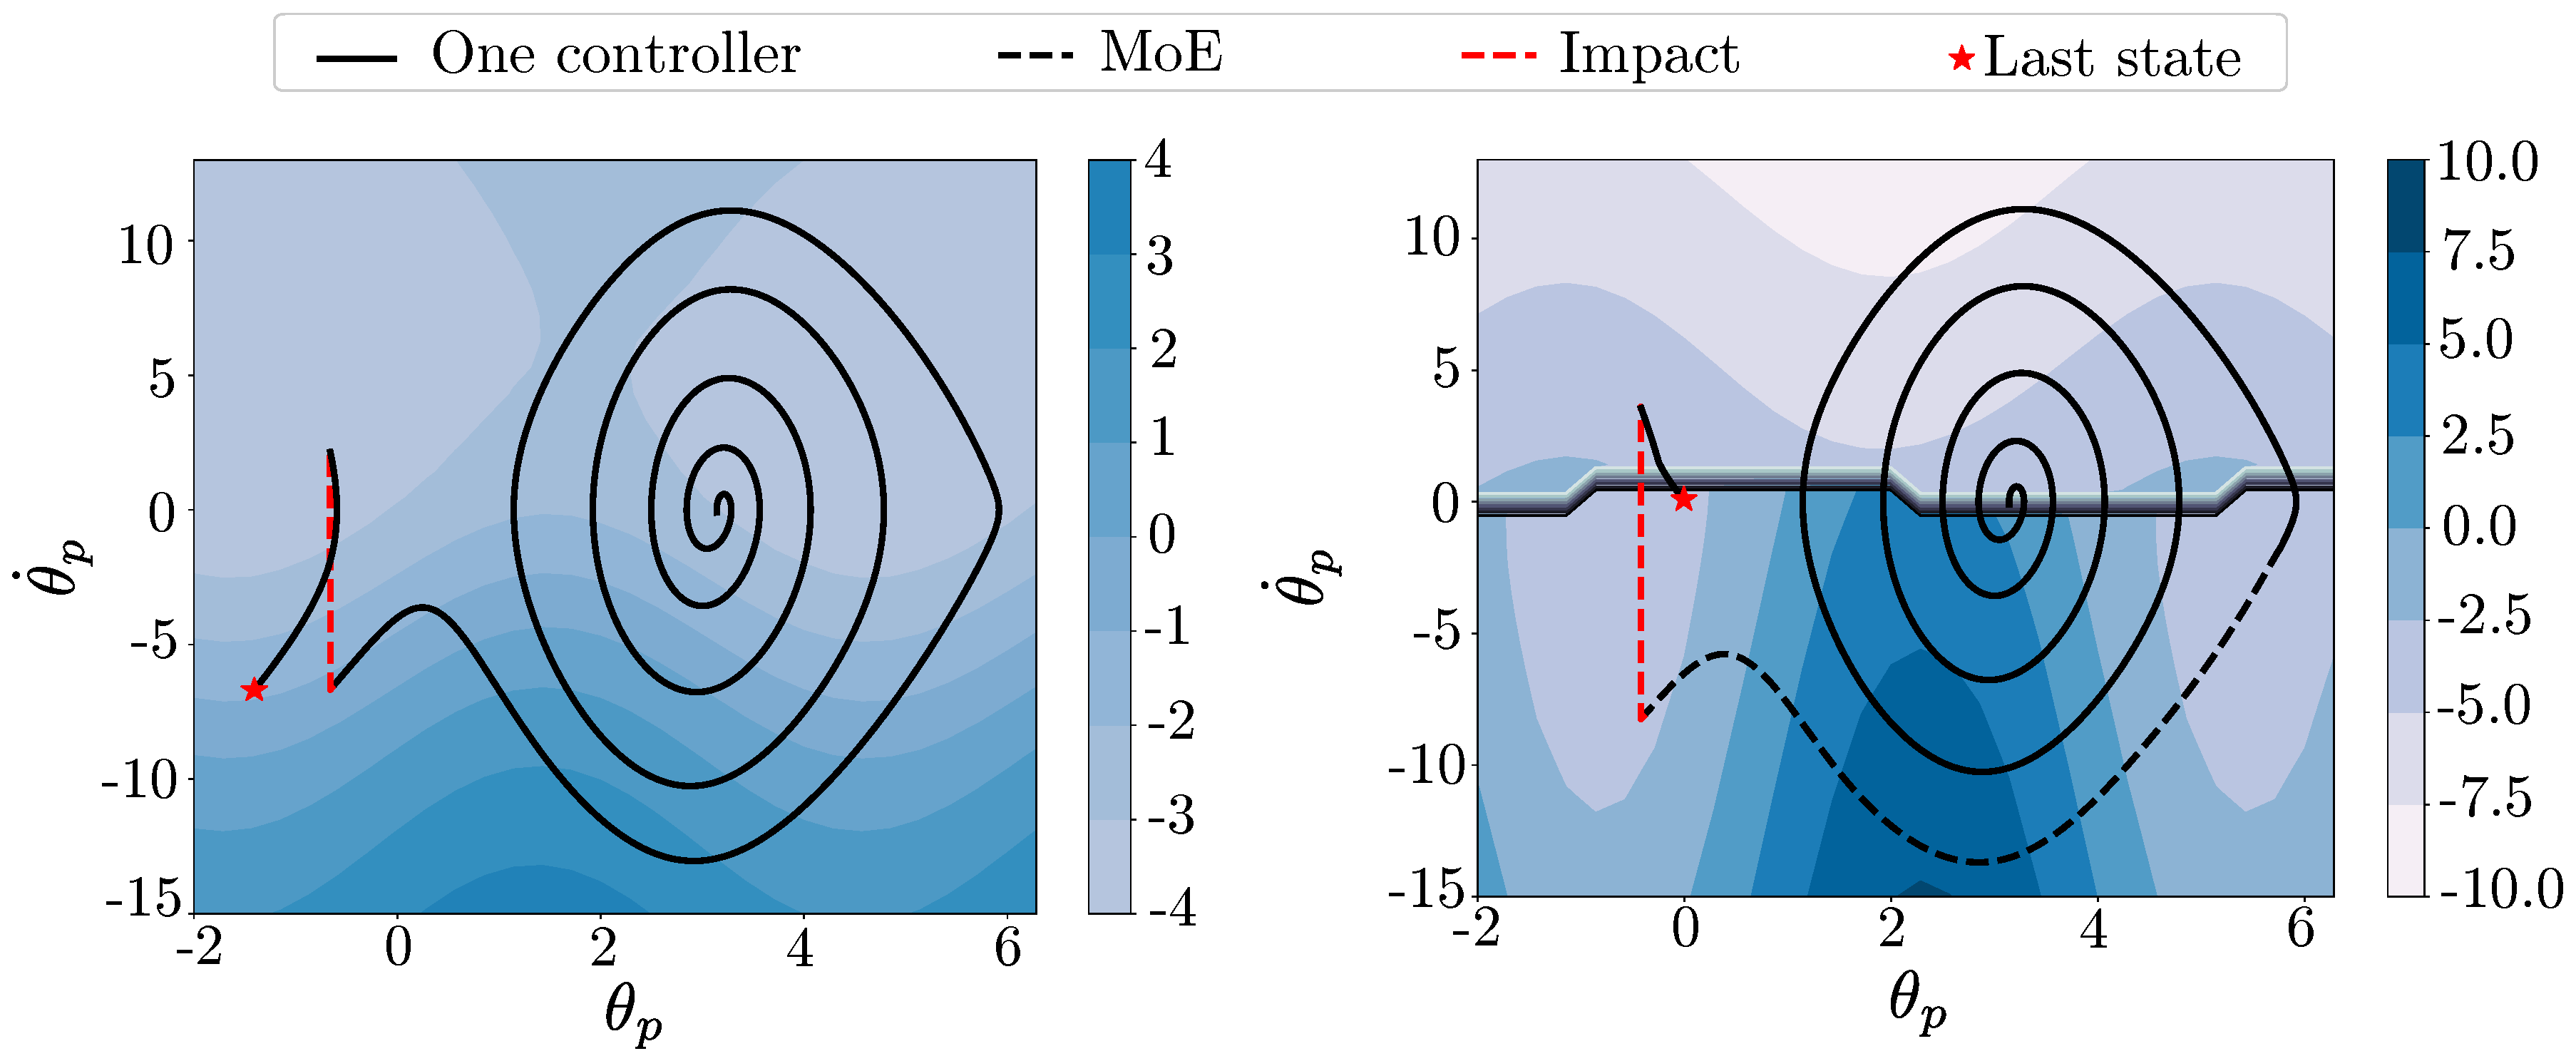
\includegraphics[width=\linewidth]{continuous_vs_MOE.eps}
    \subfloat[\label{continuous}Performance of a single controller]{\hspace{0.5\linewidth}} 
    \subfloat[\label{moe}Performance of the MoE controller]{\hspace{0.5\linewidth}}
    \caption{Comparison between MoE and a single controller}
    \label{fig:contandmoe}
\end{figure}
%
As shown in Figure~\ref{continuous}, the single controller
successfully swings up the pendulum close to the upright.
%
However, due to the length of the pendulum and the tight distance between the
walls, the pendulum inevitably impacts one of the barriers. 
%
Unfortunately, the LQR is not able to catch the pendulum post-impact, due to the
high velocity of the pendulum.
%
On the other hand, Figure~\ref{moe} shows the performance of the MoE
controller in the same scenario.
%
The MoE solution leverages the switching controllers to apply rapid braking
post-impact, which significantly lowers the velocity of the pendulum. 
%
This assists the LQR in catching the pendulum at the appropriate speed.
%
This demonstrates the advantages of switching controllers in the presence of
multi-modal contact-rich systems.
